\section{Overview of Multi-Fidelity Optimization}
%----------------------------------------------------------------------
\begin{frame}[c]{Motivating Example}

\begin{itemize}
    \item Performance of a support vector machine (SVM) on MNIST and subsets of it:\\~\\
	    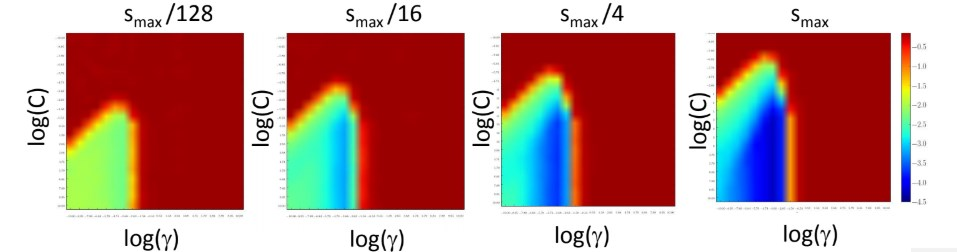
\includegraphics[width=0.9\textwidth]{w07_hpo_grey_box/images/fabolas/example_mnist.jpg}
	    \begin{itemize}
            \item Computational cost grows quadratically in dataset size $z$
            \item Error shrinks smoothly with $z$
        \end{itemize}
\bigskip
    \item Evaluations on the smallest subset (about 400 data points) cost 10\,000$\times$ less than on the full data set (50\,000 data points)
    
\end{itemize}
\end{frame}
%----------------------------------------------------------------------

%----------------------------------------------------------------------
\begin{frame}[c]{Motivating Example 2: Shorter Runs of Anytime Algorithms}

\begin{itemize}
    \item Performance with shorter runs of an anytime algorithm (such as SGD):\\~\\
\centering
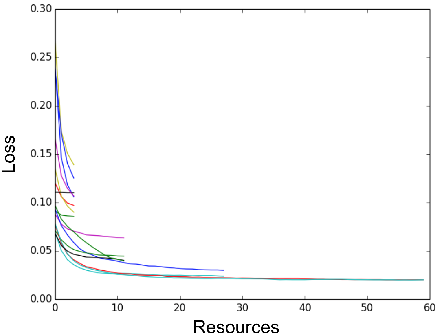
\includegraphics[width=0.5\linewidth]{w07_hpo_grey_box/images/hyperband/Figure_1_2.png}

\end{itemize}
\end{frame}
%----------------------------------------------------------------------


%----------------------------------------------------------------------
\myframe{Multi-Fidelity Optimization In General}{

Exploit cheap approximations of an expensive blackbox function $\rightarrow$ afford more configurations\\

\begin{columns}[T]
    \begin{column}{.5\textwidth}
        \myit{
            \item Idea: eliminate poor configurations early, allocate more resources to promising ones.
        }
    \end{column}
    
    \begin{column}{.4\linewidth}
        \begin{figure}
        \centering
        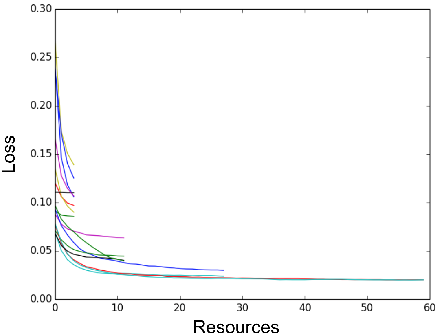
\includegraphics[width=0.9\linewidth]{w07_hpo_grey_box/images/hyperband/Figure_1_2.png}
        \end{figure}
    \end{column}
\end{columns}

\begin{columns}
    \begin{column}{.9\linewidth}
    \vspace{-10em}
\pause
\medskip
    \myit{
    	\item Possible Resources:
    	\myit{
    	    \item Runtime
    	    \item Number of epochs/iterations
    	    \item Data subset size
    	    \item Downsampled size of images in object recognition
    	    \item Depth / width of neural networks
    	    \item Number of trees 
    	    \item Number of features
    	    \item Number of cross validation folds\\~
    	    \item General concept, even in fields outside ML, e.g., fluid simulation:
    	    \myit{
    	        \item Number of particles
    	        \item Time scale of simulation
    	    }
    	}
    }
\end{column}
\begin{column}{0\linewidth}
\end{column}
\end{columns}
}


%----------------------------------------------------------------------
\begin{frame}[c]{General Remarks on Multi-Fidelity Optimization}

\myit{
    \item Often, we have a \alert{choice} which resources we use as budget
\bigskip
\pause
    \item For multi-fidelity optimization to be helpful, \alert{performance with low budgets should be informative about performance with high budgets}  
\bigskip    
\pause  
    \item In the simplest case: 
    Good with low resources $\leftrightarrow$ good with high resources.
    \myit{
        \item In practice, this is of course not always true
    }
    
}


\end{frame}



%-----------------------------------------------------------------------
\begin{frame}{How Useful is the Cheap Approximation? The Rank Correlation}

Given:
\myit{
    \item A set of configurations $\pcs = \{\conf_1, ..., \conf_n\}$
    \item The performances $f(\conf_1), ..., f(\conf_n)$ on the expensive black box
    \item The performances $g(\conf_1), ..., g(\conf_n)$ on a cheap approximation of the black box

\bigskip
\pause

}
    We compute the \alert{Spearman rank correlation} between $[f(\conf_1), ..., f(\conf_n)]$ and $[g(\conf_1), ..., g(\conf_n)]$
\myit{    
    \item If this is high (in the extreme: 1), the relative ranking of the configurations is the same on $f$ and $g$
    \myit{
        \item In that case, we can optimize cheaply on $g$ and also obtain an optimum for $f$
    }
    \item If it is low, optimizing g does not tell us anything about f

}

\bigskip
\pause
Goal: find approximations g that are very cheap but have high rank correlations with f

\end{frame}
%----------------------------------------------------------------------

%-----------------------------------------------------------------------
\begin{frame}{Questions to Answer for Yourself / Discuss with Friends}

\bigskip

\begin{itemize}
    \item \alert{Repetition.} Which cheap approximation is better in this hypothetical case?
    \myit{
        \item Downscaling images (5x cheaper, rank correlation of 0.8)
        \item Less epoch of SGD (4x cheaper, rank correlation of 0.75)
    }

\medskip
    \item \alert{Discussion.} 
    Can you think of a multi-fidelity approximation we did not discuss yet?

\end{itemize}

\end{frame}
%----------------------------------------------------------------------
%----------------------------------------------------------------------